\documentclass[aspectratio=169]{beamer}


\usepackage[utf8]{inputenc}
\usepackage{amsmath}
\usepackage{amsfonts}
\usepackage{amssymb}
\usepackage{graphicx}
\usepackage{ragged2e}  % `\justifying` text
\usepackage{booktabs}  % Tables
\usepackage{tabularx}
\usepackage{tikz}      % Diagrams
\usetikzlibrary{calc, shapes, backgrounds}
\usepackage{amsmath}
\usepackage{amssymb}
\usepackage{dsfont}
\usepackage{url}       % `\url
\usepackage{listings}  % Code listings
\usepackage[T1]{fontenc}
\usepackage{hyperref}

\usepackage{theme/beamerthemehbrs}

\author[Dashboard for ROS-based System]{}
\title{Software Development Project}
\subtitle{Dashboard for ROS-based System}
\institute[HBRS]{Hochschule Bonn-Rhein-Sieg}
\date{\today}
\subject{Test beamer}

% \thirdpartylogo{path/to/your/image}


\begin{document}
{
\begin{frame}
\titlepage
\end{frame}
}

\begin{frame}{Team Members}
\linespread{2}
\vspace*{-20mm}
	\begin{enumerate}
	\item \bf{Lokesh Veeramacheneni}
	\item \bf{Zuha Karim}
	\item \bf{Anargh Viswanath}
	\end{enumerate}
	\vspace*{5mm}
	%In the current stage of the project, the team members are yet to assume separate roles.\\ 
%\vspace*{2.5mm}	
	
\end{frame}

\begin{frame}{Problem Setting}
\vspace*{-15mm}
\begin{itemize}
\item In ROS-based system running on a robot and being controlled remotely - several processes being carried-out simultaneously.
\item Serious problem $\rightarrow$ \bf{Some process stops eg.Nodes$\rightarrow$  \textcolor{red}{Application Failure}}.
\item \textnormal {Need for efficient and real-time monitoring for remedial measures.} 
\end{itemize}

\end{frame}

\begin{frame}{Project Objective}
\vspace*{-15mm}
\justify \bf{Developing a Dashboard UI for monitoring the ROS system running on a robot remotely through a computer system via web services.}
\end{frame}

\begin{frame}{Client and Requirements}
\vspace*{-15mm}
\linespread{1.5}
\bf Client: \textnormal{Deebul Nair}\\
\textnormal{It is intended to be used by \bf{Robocup @work lab}.}

	\textnormal{Requirements:}
	\begin{enumerate}
	\item \textnormal{Should be implemented inside Cockpit - open web-based interface for servers}
	\item \textnormal{Smooth monitoring of ROS and Robot's system metrics.}
	\item \textnormal{Effortless visualization of ROS Nodes.}
	\item \textnormal{Start and kill the ROS nodes(if possible).}
	\end{enumerate}
	
\end{frame}


\begin{frame}{Main Components of Software}
\vspace*{-10mm}
\linespread{1.5}
\begin{enumerate}
	\item \textbf{Cockpit} - Integrated open web-based interface for GNU/Linux server.\\ \textbf{Features of Cockpit:}
	\begin{itemize}
	\item Monitor and administer several servers at the same time.
	\item Uses the system’s normal user logins and privileges by default. 
	\item Network login supported.
	\item When inactive, no extra load on the server.
	\item Inbuilt packages show the status of the system.
	\item Embedded terminal present within interface.
	\end{itemize}
	\item \justify \textbf{ROS Kinetic} - Installed on the robot which has to be monitored.
\end{enumerate}
	
\end{frame}

\begin{frame}{Coding standards}
\vspace*{-25mm}
\linespread{2}
\begin{enumerate}
	\item \textbf{Python}
	\begin{itemize}
	\item PEP8
	\end{itemize}
	\item \textbf{Javascript}
		\begin{itemize}
	\item Google JavaScript Style Guide
	\end{itemize}
\end{enumerate}
	
\end{frame}

\begin{frame}{Organization of Work}
\vspace*{-15mm}
\linespread{2}
	\begin{itemize}
	\item Project development, management and release carried out through Github.
	\item Each member has a separate branch for development.
	\item Master branch has reviewed components merged from branches.
	\item Issues, Sprints and progress also being placed.
	\item  \href{https://github.com/lokeshveeramacheneni/Software-Development-Project/tree/master}{\underline{Link to Github Repository}} 
	\end{itemize}
	
\end{frame}

\begin{frame}{Project Implementation}
\begin{figure}
  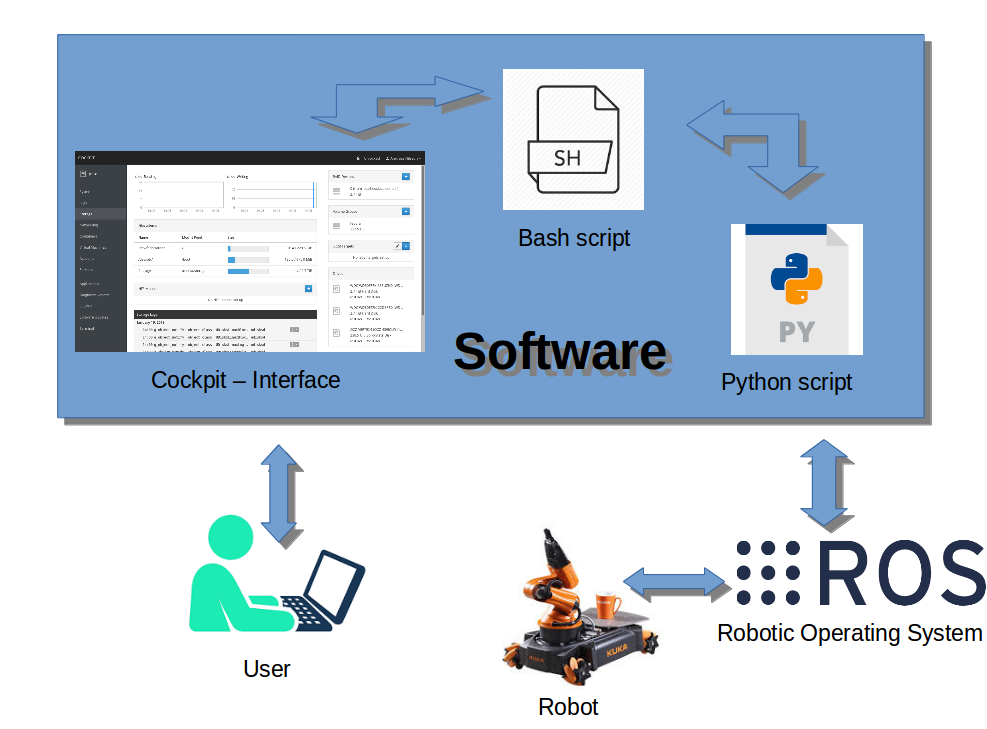
\includegraphics[width=0.6\linewidth]{Working.png}
  \caption{Working of Software}
  \label{fig: Implementation}
\end{figure}
\end{frame}

\begin{frame}{Dashboard Layout}
\begin{figure}
  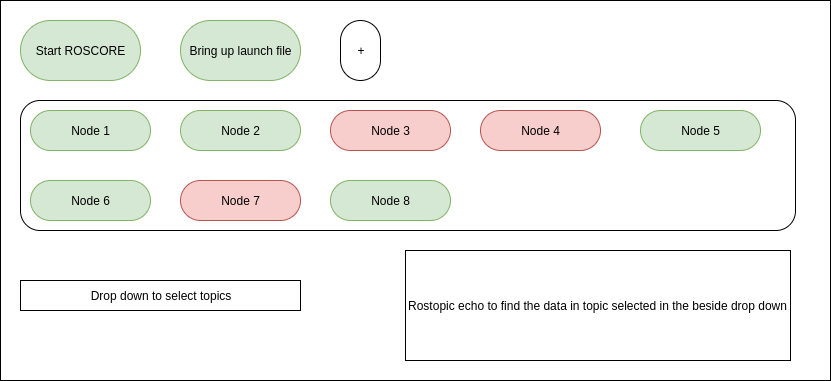
\includegraphics[width=0.8\linewidth]{Layout.png}
  \caption{Layout of Dashboard}
  \label{fig: Layout}
\end{figure}
\end{frame}

\begin{frame}{Module I}
% Here Lokesh will put his work and explain
Start and Kill Rosmaster.
Selecting Launch file Description.
\end{frame}

\begin{frame}{Module II}
% Here Anargh will put his work and explain
Getting the node status from launcher and display.
\end{frame}

\begin{frame}{Module III}
% Here Zuha will put his work and explain
Getting the rostopics and diplaying details.
\end{frame}

\begin{frame}{Problems occured during development}
\vspace*{-15mm}
\linespread{2}
	\begin{itemize}
	\item \bf Creating packages inside ROS.
	\item \bf Connecting Cockpit to ROS.
	\item \bf Starting and Killing ROS master from Dashboard.
	\item \bf Getting Node status of launch file inside cockpit and display. 
	\item \bf Getting Topics as list and display.
	\end{itemize}
\end{frame}

\begin{frame}{Development Status - Capabilities}
\vspace*{-15mm}
\linespread{2}
	\begin{itemize}
	\item \bf Easy installation of Cockpit and Dashboard inside system.
	\item \bf The Dashboard can start and kill ROS master.
	\item \bf Display the status of ROS nodes inside selected launch file. 
	\item \bf Display information about the ROS topics.
	\end{itemize}
\end{frame}

\begin{frame}{Development Status - Limitations}
\vspace*{-15mm}
\linespread{2}
	\begin{itemize}
	\item Certain GUI based nodes not launched from Dashboard.
	\item The feature for starting and killing nodes not developed.
	\end{itemize}
\end{frame}

\begin{frame}{Development Status - Wish List}
\vspace*{-15mm}
\linespread{2}
	\begin{itemize}
	\item \bf \textcolor{green}{Small wish} - Incorporating the feature for starting and killing nodes for better usage.
	\item \bf \textcolor{blue}{Big Dream} - Dashboard able to control all aspects of ROS.
	\end{itemize}
\end{frame}

\begin{frame}{Demonstration}
\vspace*{-15mm}
\center \bf{A brief demonstration of the system}
\end{frame}

\begin{frame}{Summary}
\vspace*{-15mm}
\linespread{2}
	\begin{itemize}
	\item Implememted Software-development practices for developing a Dashboard for monitoring ROS-based system via web services. 
	\item Completed the basic package for the client's initial requirements.
	\item The software can be extended and improved through further work.
	\end{itemize}
\end{frame}

\end{document}
